\documentclass{article}
\usepackage[final,dblblindworkshop]{neurips_2026}
\workshoptitle{AI for Drug Discovery: Bridging the Translation Gap}

\usepackage[utf8]{inputenc}
\usepackage[T1]{fontenc}
\usepackage[hidelinks]{hyperref}
\usepackage{url}
\usepackage{booktabs}
\usepackage{amsmath,amsfonts,amssymb}
\usepackage{microtype}
\usepackage{xcolor}
\usepackage{graphicx}
\graphicspath{{figures/}{../}}

\title{Active Learning for Molecular-Docking Algorithm Selection under Heterogeneous Runtime}
\author{Sean Wan \qquad Jiabao Brad Wang \qquad Mustafa Misir\\
Duke Kunshan University}

\begin{document}
\maketitle

\begin{abstract}
Training an algorithm selector for structure-based drug discovery typically requires evaluating every docking method on every protein--ligand complex.
We formulate this costly matrix construction as closed-loop active learning, where each retrospective query reveals a recorded docking outcome and runtime.
Using MolAS, we evaluate cell-wise active acquisition and compare five predicted-runtime transformations of Mean-UCB, fitting runtime models only to previously observed training-pool runtimes.
Across seven docking methods and five held-out folds, selective acquisition recovers decision-useful training data without exhaustive evaluation.
No evaluated formulation consistently leads across the reported endpoints and budgets: runtime transformations reshape algorithm allocation and can defer expensive evidence, while matrix-quality metrics do not consistently track held-out performance.
These results provide an empirical reference for resource-aware active learning in molecular docking.
\end{abstract}

\noindent\textbf{Keywords:} active learning; algorithm selection; molecular docking; protein--ligand interactions; drug discovery; runtime-aware acquisition; structure-based virtual screening.

\section{Introduction}
AI-driven structure-based drug discovery increasingly orchestrates portfolios of classical and learned docking methods whose performance varies across protein--ligand complexes. Automated algorithm selection (AS) exploits this complementarity by choosing a suitable method for each complex~\citep{rice1976algorithm,kerschke2019automated}, using molecular descriptors, graphs, or pretrained representations~\citep{chen2023algorithm,cao2025mc,wang2026molecular}. Training a selector, however, ordinarily requires executing every docking method on every training complex to construct a complete performance matrix. We instead formulate this process as resource-constrained computational experimental design: active learning (AL) selects a complex--algorithm cell, acquires its docking outcome, updates the matrix model, and repeats~\citep{cohn1996active,tharwat2023survey,huseljic2026refine}.

This setting differs from docking AL under a fixed workflow~\citep{graff2021accelerating,marin2024regression}: each query identifies both the protein--ligand complex and the docking method, and the resulting partial matrix must support decisions on unseen complexes. Our technical basis is active matrix completion~\citep{misir2019active}. Previous studies explored uncertainty-guided and runtime-aware acquisitions for AS in combinatorial optimization~\citep{volpato2019active,kus2026frugal}; here, we investigate cell-wise acquisition for molecular-docking AS.

\noindent\textbf{RQ1.} To what extent can cell-wise AL reduce molecular-docking evaluations while preserving held-out MolAS decision quality?

Query count alone is insufficient because docking runtime varies by complex and algorithm and is unknown before execution. Cost-blind AL may select informative but slow runs, whereas utility-per-cost rules may defer expensive yet selector-relevant evidence.

\noindent\textbf{RQ2.} How do alternative predicted-runtime transformations change algorithm allocation and the downstream performance--cost frontier?

We empirically evaluate cell-wise acquisition on MolAS~\citep{wang2026molecular} through historical replay, comparing Mean-UCB with five predicted-runtime acquisition-score formulations. Our results address a translation challenge in AI for drug discovery: partial acquisition can support useful selectors, but the effect of cost awareness depends on formulation and budget, and computational proxies do not consistently track downstream molecular decisions. Code and data are being prepared for public release.

\section{Background}
\paragraph{Active performance acquisition for algorithm selection.}
Standard AL generally treats an instance-level label as the query unit~\citep{tharwat2023survey}, whereas AS admits instance--algorithm outcomes. Active matrix completion (AMC) selects entries of an incomplete performance matrix to reveal~\citep{chakraborty2013active}, and supervised AMC can incorporate acquisition cost~\citep{huang2018afasmc}. AMC has been applied directly to AS~\citep{misir2019active}; related work studies instance-level active acquisition for time-expensive AS~\citep{volpato2019active}, while Frugal AS combines uncertainty-based acquisition with learned timeout models~\citep{kus2026frugal}. These studies motivate selective acquisition under limited computational budgets. Recent AL work also highlights the influence of pool management and evaluation protocols on observed performance~\citep{huseljic2026refine}. Low reconstruction error need not preserve algorithm rankings or downstream molecular decisions; MolAS provides a structure-based virtual-screening backend for evaluating this distinction~\citep{wang2026molecular}.

\paragraph{Cost-aware acquisition under heterogeneous runtime.}
Cost-sensitive AL trades informativeness against annotation or execution cost~\citep{tomanek2010comparison,gao2020cost}. Return-on-investment rules rank queries by estimated benefit per unit cost~\citep{haertel2015analytic}; more generally, $U/C^\gamma$ interpolates between cost-blind utility ($\gamma=0$) and direct utility per cost ($\gamma=1$). Pareto analyses characterize utility--cost trade-offs~\citep{guinet2020pareto}, while budgeted Bayesian optimization studies non-myopic acquisition under unknown evaluation costs~\citep{astudillo2021multi}. Batch acquisition adds potential redundancy among individually attractive queries, motivating joint strategies such as BatchBALD~\citep{kirsch2019batchbald}. In molecular docking, favoring inexpensive cells can systematically reshape which algorithms contribute training outcomes. We therefore evaluate runtime-aware acquisition through realized cost, allocation, and held-out MolAS performance, alongside matrix diagnostics.

\section{Methodology}
\subsection{Closed-loop active acquisition of AS training data}
Let $\mathcal I=\{i_1,\ldots,i_n\}$ denote training-pool protein--ligand complexes and $\mathcal A=\{a_1,\ldots,a_m\}$ a portfolio of $m$ docking algorithms. Their strict performance and acquisition cost matrices are
\begin{equation}
\mathbf Y\in[0,1]^{n\times m},
\qquad
\mathbf C\in\mathbb R_{+}^{n\times m}.
\end{equation}
In our retrospective evaluation, querying $q=(i,a)$ reveals its recorded docking score and runtime, $(Y_{ia},C_{ia})$. At round $t$, only cells in $\Omega_t$ are observed; the remaining pool is $\mathcal U_t=(\mathcal I\times\mathcal A)\setminus\Omega_t$. Paired trajectories share a runtime-blind $1\%$ warm start, distributed as evenly as possible across algorithms.

Given $\Omega_t$, iterative low-rank SVD completion~\citep{mazumder2010spectral} estimates unobserved performance. An ensemble of ranks $\mathcal K=\{1,2,3,5\}$ produces
\begin{equation}
\mu^Y_{ia}=\frac{1}{|\mathcal K|}\sum_{k\in\mathcal K}\widehat Y^{(k)}_{ia},
\qquad
\sigma^Y_{ia}=\operatorname{SD}_{k\in\mathcal K}\bigl(\widehat Y^{(k)}_{ia}\bigr).
\end{equation}
These ranks provide different low-rank hypotheses for the seven-column matrix. An acquisition rule assigns $\alpha_t(i,a)$ to each unqueried cell. Selected cells are revealed, and the completion and runtime models are updated. Scores are reranked after batches of at most 50 queries, truncated at checkpoint boundaries; this reduces refitting frequency while holding scores fixed within a batch. A completed training matrix is exported at every integer acquisition percentage from $1\%$ to $100\%$. No new docking jobs are executed.

We evaluate 3,179 Binding-MOAD complexes~\citep{hu2005binding}, as in MolAS~\citep{wang2026molecular}, with seven algorithms: Smina~\citep{koes2013smina}, AutoDock Vina~\citep{trott2010vina}, DiffDock and DiffDock-L~\citep{corso2023diffdock,corso2024diffdockl}, SurfDock~\citep{cao2025surfdock}, GNINA~\citep{mcnutt2021gnina}, and Uni-Mol Docking V2~\citep{alcaide2025unimol}. MolAS combines RMSD with a PoseBusters-validity gate~\citep{buttenschoen2024posebusters}. We retain the original five outer folds. At each evaluated acquisition checkpoint, MolAS is trained on the completed matrix for that fold's training complexes: queried cells retain observed scores, while unqueried cells receive SVD estimates. Completion and supervised model fitting use the $80\%$ training split; the held-out fold is reserved for evaluation. The downstream comparison uses the seed-0 acquisition archive with matched warm starts; summaries are over outer folds, not independent acquisition/selector-seed replications.

We report valid-pose success below $1$ and $2$~\AA, an AS composite score, and closure of the single-best-solver (SBS) to virtual-best-solver (VBS) gap. Matrix MAE, row-wise Spearman $\rho$, pairwise concordance, NDCG@$3$, and decision regret are diagnostics. Reported cost sums recorded docking-job runtimes, including the warm start, and excludes feature/model-fitting overhead and parallel scheduling. Fold summaries are descriptive, without confidence intervals or significance tests; overlapping training splits are not independent replications.

\subsection{Mean-UCB acquisition utility}
To examine runtime handling within a common acquisition framework, we use Mean-UCB throughout the comparison. Adapted from \citet{qin2025active}, it combines predicted performance with ensemble dispersion:
\begin{equation}
U_t(i,a)=\mu^Y_{ia}+\beta\sigma^Y_{ia}.
\end{equation}
We fix $\beta=1$ and the predictive model class across policies; each policy updates its predictions from its own acquired observations. Dispersion across SVD ranks is a heuristic uncertainty measure, not a calibrated confidence bound.

\subsection{Runtime-aware acquisition from observed costs}
Unqueried runtime is predicted from information available before revealing that cell:
\begin{equation}
\widehat C_{ia}=h_t(\mathbf x_i,\mathbf d_i,\mathbf e_a),
\end{equation}
where $\mathbf x_i$ concatenates protein and ligand representations, $\mathbf d_i$ contains four physical descriptors, and $\mathbf e_a$ is a one-hot algorithm identifier. A two-hidden-layer MLP with widths $(32,16)$ is trained on $\log(1+C_{ia})$ using only runtimes revealed in $\Omega_t$. Predictions are transformed back to seconds and clipped to the observed-runtime 5th--95th percentile bounds $[\ell_t,u_t]$, with numerical safeguards. Clipping limits extreme predictions but can also underrepresent runtime tails. Unqueried runtimes and full-matrix runtime statistics are excluded from acquisition. Ranks, reranking interval, $\beta$, and clipping define the evaluated configuration; their sensitivity has not been established.

All utility ranks and cost normalizations use the current unqueried training pool $\mathcal U_t$, across algorithms, separately for each policy. Let $\widetilde U_t=\max\{10^{-3},\operatorname{rank}_{\mathrm{avg}}(U_t)/|\mathcal U_t|\}$, using ascending ranks with averaged ties. For a candidate-cost vector $c$, define
\begin{equation}
\mathcal S_t[c](q)=1+4\frac{c(q)-\min_{r\in\mathcal U_t}c(r)}
{\max_{r\in\mathcal U_t}c(r)-\min_{r\in\mathcal U_t}c(r)}.
\end{equation}
If the extrema are numerically equal, $\mathcal S_t[c]=1$. Set $\widetilde C=\mathcal S_t[\widehat C]$. With cell indices suppressed, we compare
\begin{align}
\alpha_{\mathrm{plain}}&=U_t,
&
\alpha_{\mathrm{direct}}&=\frac{U_t}{\widehat C+\epsilon},
&
\alpha_{\mathrm{sqrt}}&=\frac{\widetilde U_t}{\sqrt{\widetilde C}},
\nonumber\\
\alpha_{\mathrm{log}}&=\frac{\widetilde U_t}{\log(1+\widetilde C)},
&
\alpha_{\mathrm{tier}}&=\frac{\widetilde U_t}{g_5(\widehat C)},
&
\alpha_{\mathrm{unc}}&=\frac{\widetilde U_t}{\sqrt{\widetilde C^+}}.
\end{align}
Here $\epsilon=10^{-6}$, and $g_5$ assigns costs to five candidate-pool quantile tiers, with boundary ties assigned to the lower tier. For runtime uncertainty, three predictors are individually transformed and clipped; their mean $\mu^C$ and population SD $\sigma^C$ give $C^+=\operatorname{clip}(\mu^C+\sigma^C,\ell_t,u_t)$ and $\widetilde C^+=\mathcal S_t[C^+]$. Other cost-aware policies use one predictor. The mean-plus-SD penalty is heuristic, not a calibrated runtime bound.

Direct cost-utility uses raw $U_t$ and predicted seconds; the other cost-aware variants use percentile utility and transformed costs. We therefore compare complete acquisition-score formulations sharing a Mean-UCB definition, rather than isolating the denominator alone. The acquisition logarithm is distinct from the log-runtime regression target.

\section{Results}
\subsection{Partial active acquisition produces decision-useful AS data}
Figure~\ref{fig:gap-closure} reports held-out SBS--VBS gap closure against cumulative realized docking runtime. Across the three endpoints, acquisition recovers substantial decision quality before exhaustive matrix completion. Plain Mean-UCB is competitive at low and intermediate realized cost, while runtime-aware variants exhibit different trajectories for valid RMSD below $1$~\AA, valid RMSD below $2$~\AA, and the AS composite score.

No evaluated policy leads across all endpoints and budget regions. Some partial-matrix checkpoints match or exceed full-matrix MolAS, although fold trajectories vary substantially, particularly at small budgets. These comparisons do not establish that omitting labels improves generalization.

\begin{figure}[t]
\centering
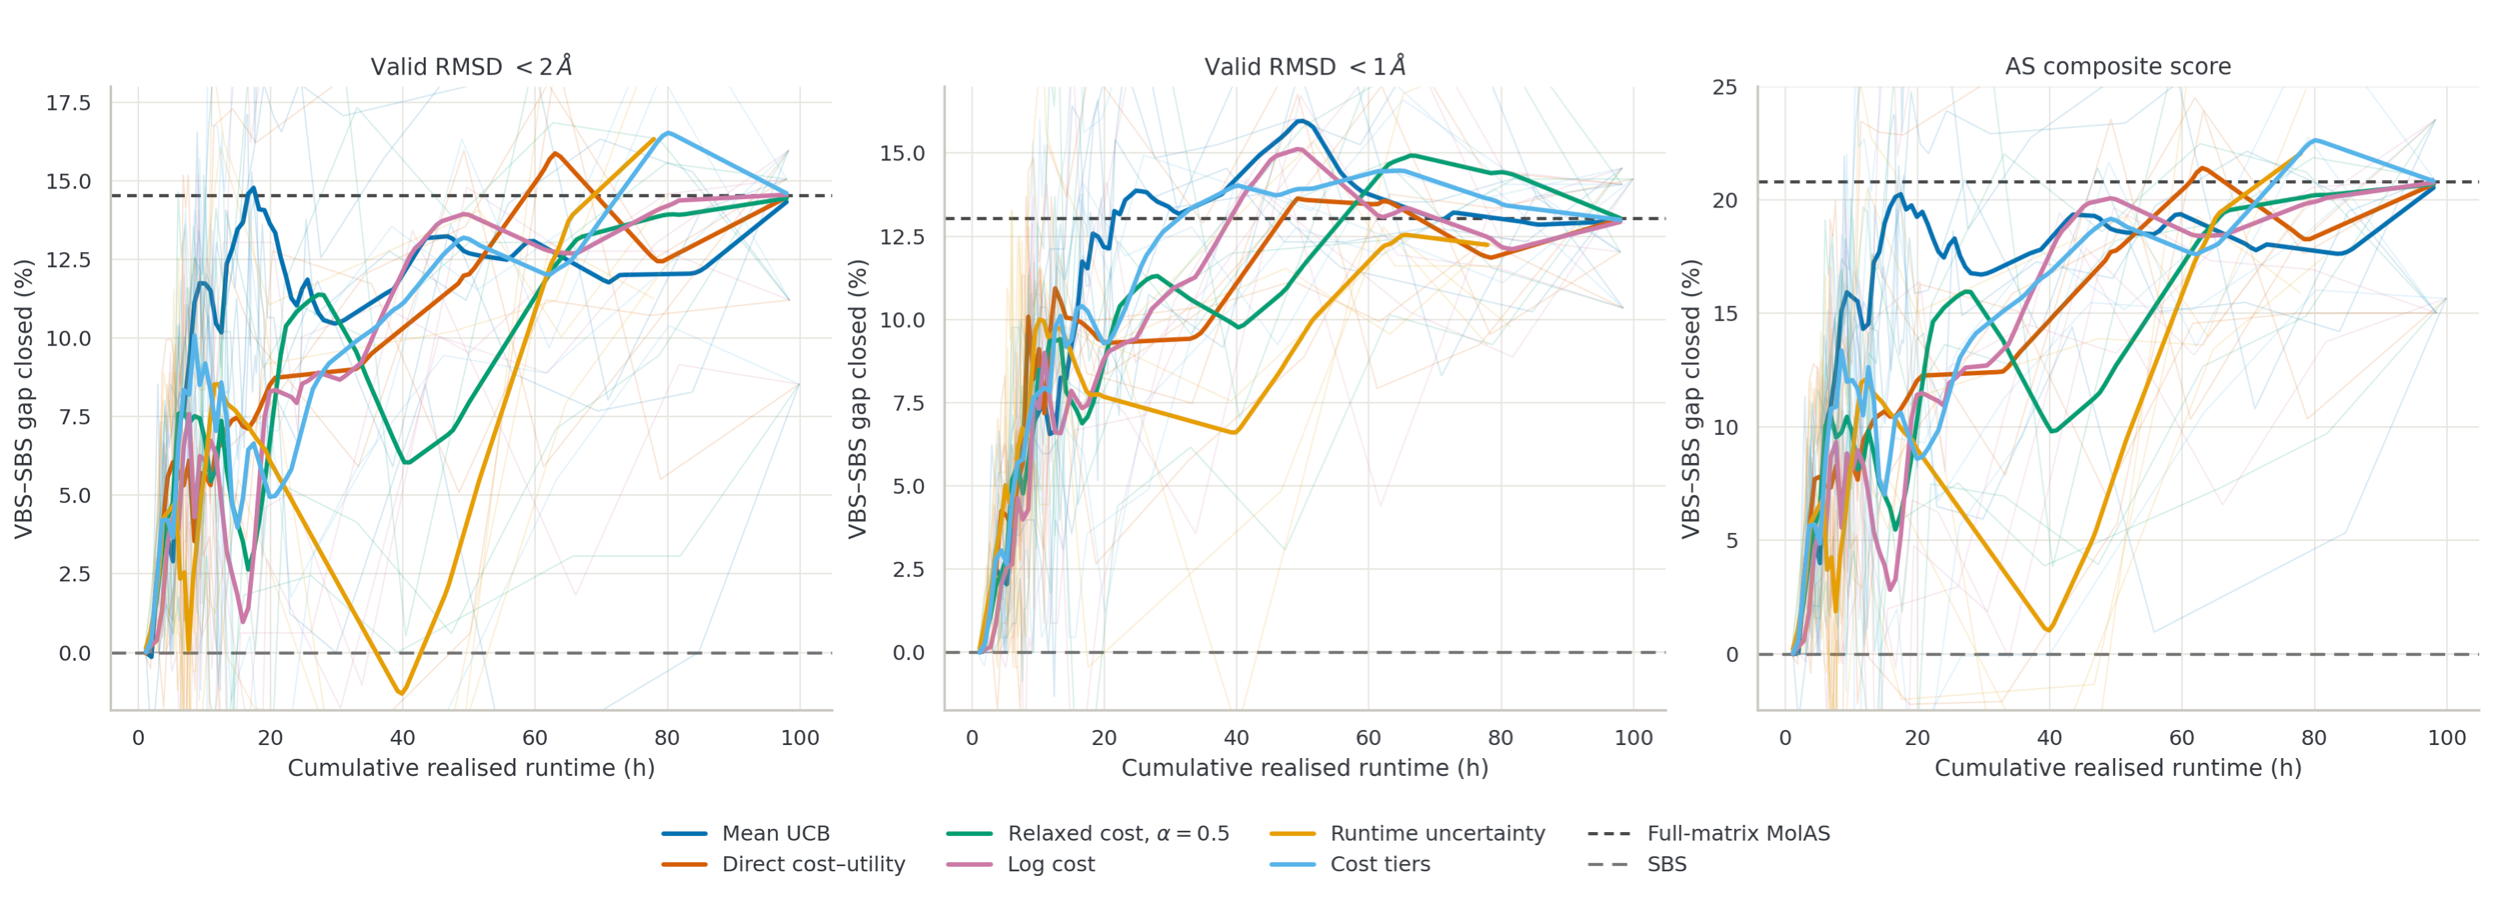
\includegraphics[width=\linewidth]{Fig1.png}
\caption{Held-out MolAS SBS--VBS gap closure versus cumulative realized runtime. Bold curves show descriptive five-fold summaries; light curves show fold trajectories. Dashed lines denote SBS and full-matrix MolAS.}
\label{fig:gap-closure}
\end{figure}

\subsection{Cost awareness changes the frontier, but not uniformly}
Despite sharing a Mean-UCB definition, folds, warm starts, completion model, and update schedule, the formulations yield different performance--cost trajectories. Because utility and cost scalings differ, denominator transformations alone do not establish an ordering of cost pressure. None consistently leads across the reported endpoints and budgets. Runtime-aware policies bring inexpensive algorithms forward and defer some expensive queries (Appendix~\ref{app:acquisition-allocation}); greater acquisition volume does not consistently yield better held-out performance.

Figure~\ref{fig:metric-association} shows that associations between matrix diagnostics and held-out MolAS gap closure vary with acquisition stage and endpoint. Decision regret exhibits a positive association over several intermediate-cost regions, particularly for valid RMSD below $1$~\AA, whereas row-wise Spearman $\rho$ is frequently weak or negative. NDCG@$3$ is informative in some regions but unstable across endpoints. Fold-level trajectories also vary, especially early in acquisition. No evaluated diagnostic consistently tracks downstream quality across this comparison.

Runtime prediction adds another source of uncertainty. Appendix~\ref{app:predicted-runtime} documents early underprediction for Uni-Mol and both DiffDock variants, and a long positive error tail for AutoDock Vina. Realized runtime, allocation, matrix diagnostics, and held-out quality provide complementary evidence; these associations do not isolate the causal contribution of prediction errors.

\begin{figure}[t]
\centering
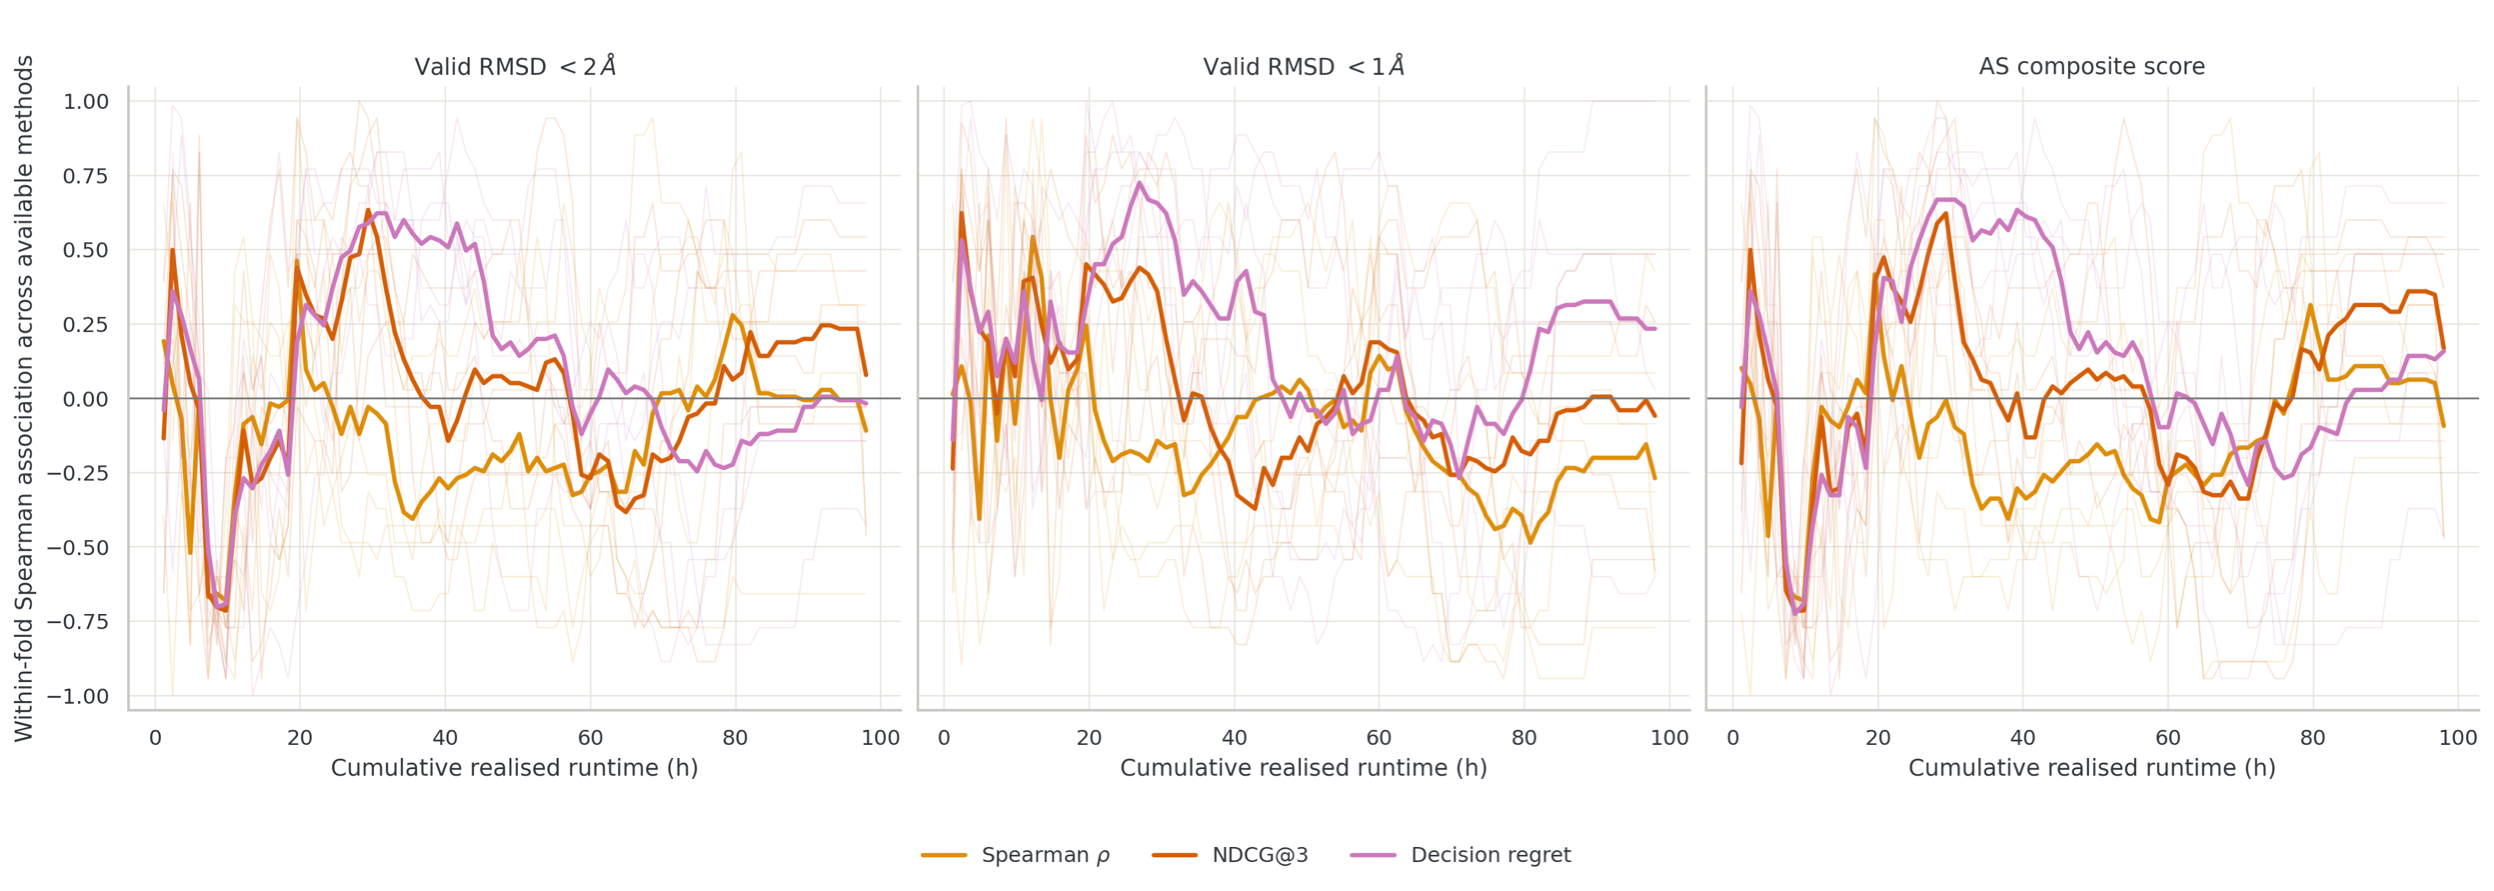
\includegraphics[width=\linewidth]{Fig2.png}
\caption{Within-fold Spearman associations across available acquisition policies between matrix diagnostics and held-out MolAS gap closure over realized runtime. Colors identify diagnostics; light curves show fold-level associations and bold curves summarize their trends.}
\label{fig:metric-association}
\end{figure}

\section{Discussion, Limitations, and Conclusion}
\noindent\textbf{Discussion.}
Runtime-aware acquisition changes both how many cells can be queried within a budget and which docking algorithms contribute evidence. In the evaluated portfolio, cost-aware policies bring inexpensive algorithms forward and defer some expensive queries, increasing acquisition volume without consistently improving held-out MolAS quality. Bridging computational benchmarks to drug-discovery decisions requires evaluation by realized runtime, allocation, matrix fidelity, and held-out molecular decision quality. Reconstruction diagnostics remain useful for assessing imputation but are insufficient proxies for selector quality.

For practical use, specify the endpoint and budget in advance; choose acquisition and stopping settings on separate validation complexes, counting their labeling cost, and reserve test folds for final evaluation. Monitor per-engine runtime errors and acquisition coverage alongside selector quality. These recommendations are not a validated deployment procedure.

\noindent\textbf{Limitations and Future Work.}
We study one curated benchmark and seven algorithms, using SVD completion and myopic Mean-UCB formulations. Random-cell, pure-uncertainty, and joint-batch baselines are absent; completion-induced bias is not separately assessed. Runtime is hardware-dependent; our sequential cost model does not address parallel scheduling, failures, or timeouts. Unqueried outcomes remain hidden during acquisition. Broader baselines, completion models, statistical characterization, sensitivity studies, runtime calibration, additional datasets/portfolios, and prospective validation are detailed in Appendix~\ref{app:next-steps}.

\noindent\textbf{Conclusion.}
Partial docking evaluations can construct decision-useful AS training data. No evaluated formulation consistently leads across the reported endpoints and budgets. Cost awareness changes both computation and the evidence available to the selector. Observed-runtime fitting, realized-cost reporting, allocation audits, and held-out MolAS evaluation together provide an empirical reference for runtime-aware acquisition in molecular docking.

\bibliographystyle{plainnat}
\bibliography{citations}
\clearpage
\appendix

\section{Runtime heterogeneity and the mechanism of cost-aware acquisition}

\subsection{Runtime scale and recoverability}
\label{app:predicted-runtime}

Algorithm identity provides a strong first-order cost signal (Figure~\ref{fig:runtime_dist}), but a single average does not describe the observed within-engine tails. Uni-Mol and the two DiffDock variants are consistently costly, whereas Smina and SurfDock are usually cheap. AutoDock Vina is a consequential exception: its median is below those of Uni-Mol and the DiffDock variants, but its upper tail spans orders of magnitude. Cost-aware acquisition therefore encounters both between-algorithm scale differences and within-algorithm tail risk. AutoDock Vina has a median runtime of $12$\,s but a mean of $48.4$\,s and accounts for $42.7$ of the $123.2$ hours required by the full matrix.

\begin{figure}[!htb]
\centering
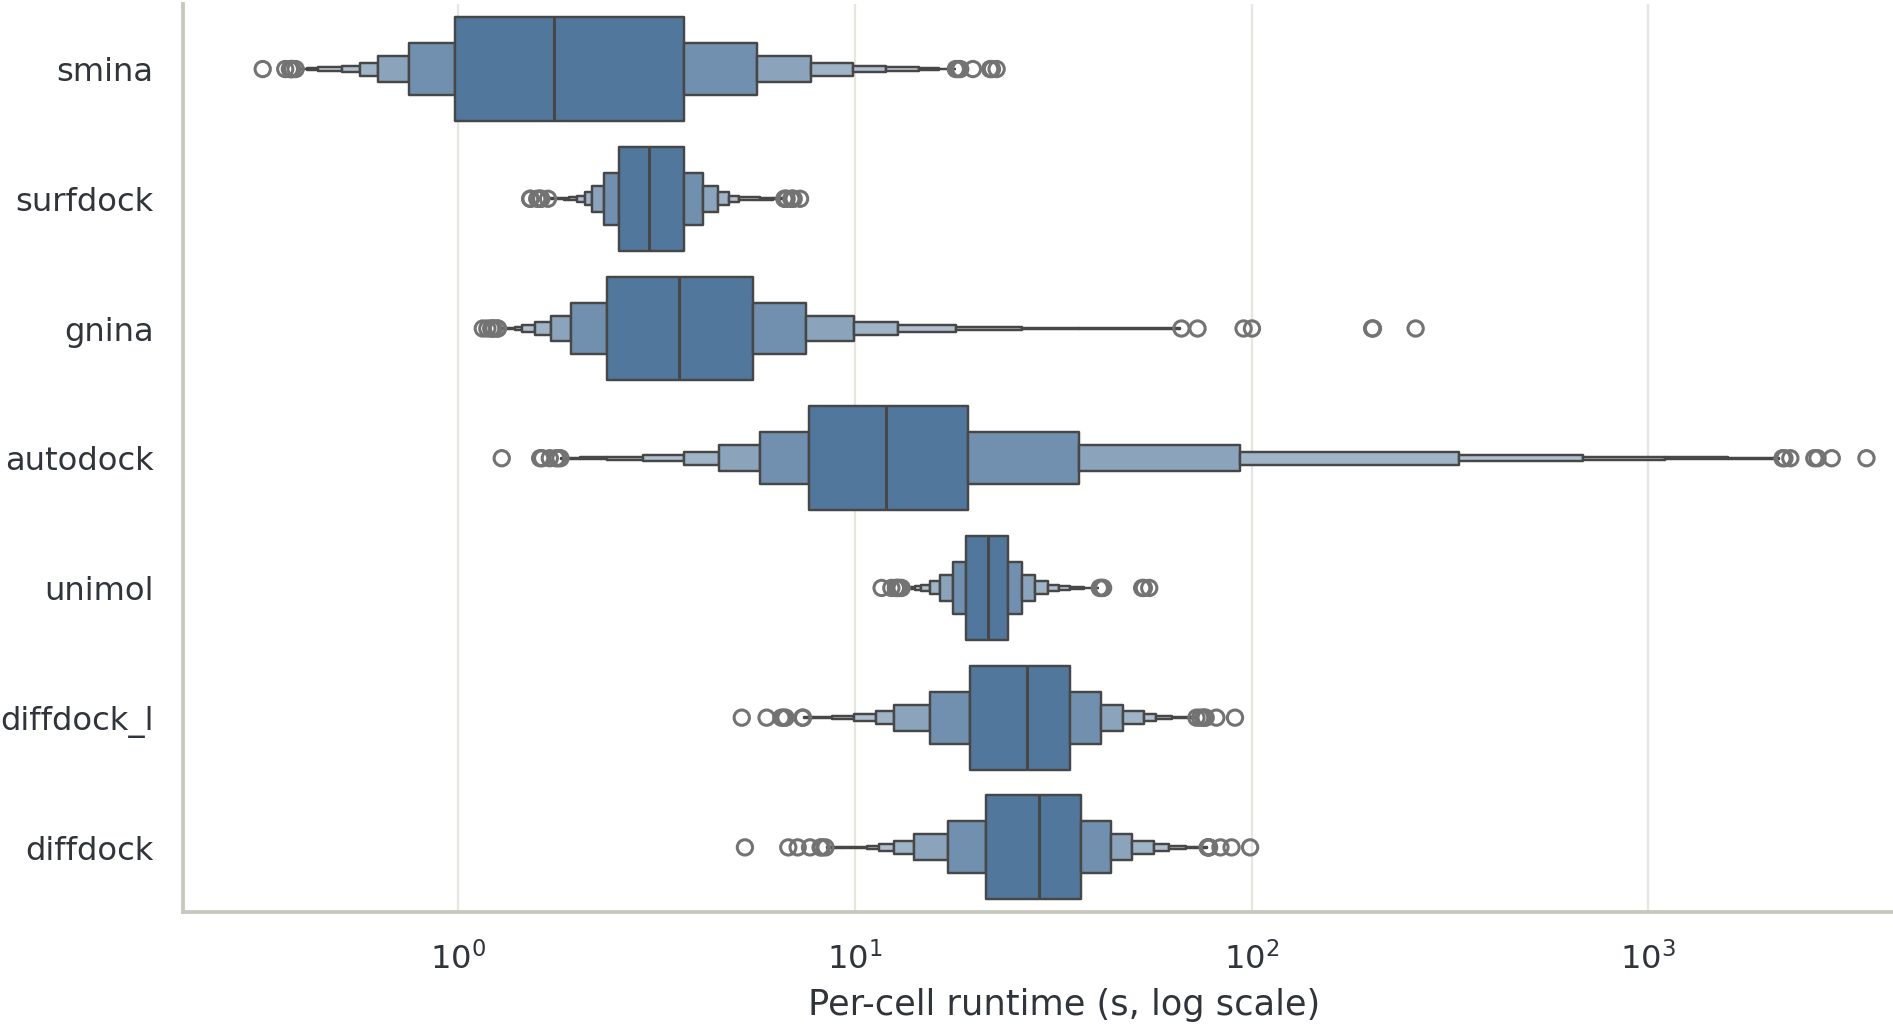
\includegraphics[width=\linewidth]{figures/runtime_distribution-REV.png}
\caption{Per-cell runtime distributions across 3,179 MOAD-curated complexes.}
\label{fig:runtime_dist}
\end{figure}

\begin{figure}[!htb]
\centering
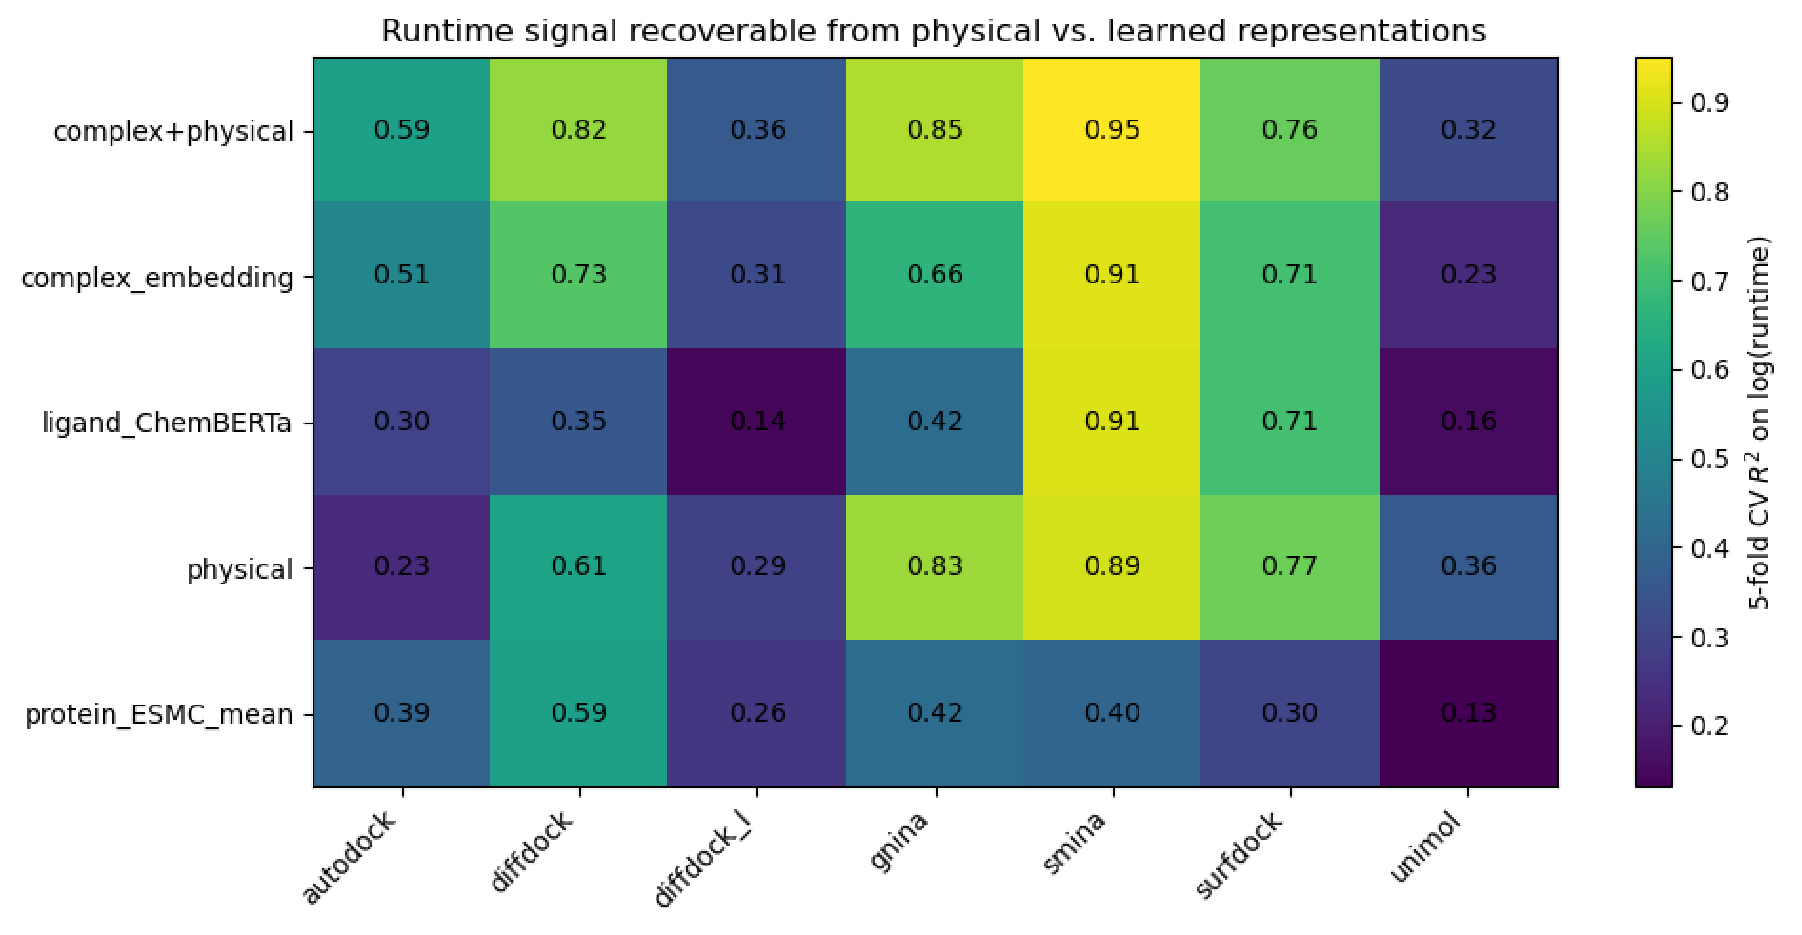
\includegraphics[width=\linewidth]{figures/cost_predictability.pdf}
\caption{Mean five-fold cross-validation $R^2$ from engine-specific ridge probes on log runtime.}
\label{fig:cost_predictability}
\end{figure}

The ridge probes in Figure~\ref{fig:cost_predictability} show that runtime is linearly predictable from the available features for some engines under this diagnostic protocol. The combined complex representation and physical descriptors explain log runtime well for Smina, GNINA, DiffDock, and SurfDock, but only moderately for AutoDock Vina and weakly for DiffDock-L and Uni-Mol. Adding representations is not uniformly beneficial. A low probe $R^2$ does not establish that nonlinear prediction is impossible. Conversely, probe performance does not validate the calibration of the acquisition-time MLP trained on selectively observed runtimes.

\begin{figure}[!htb]
\centering
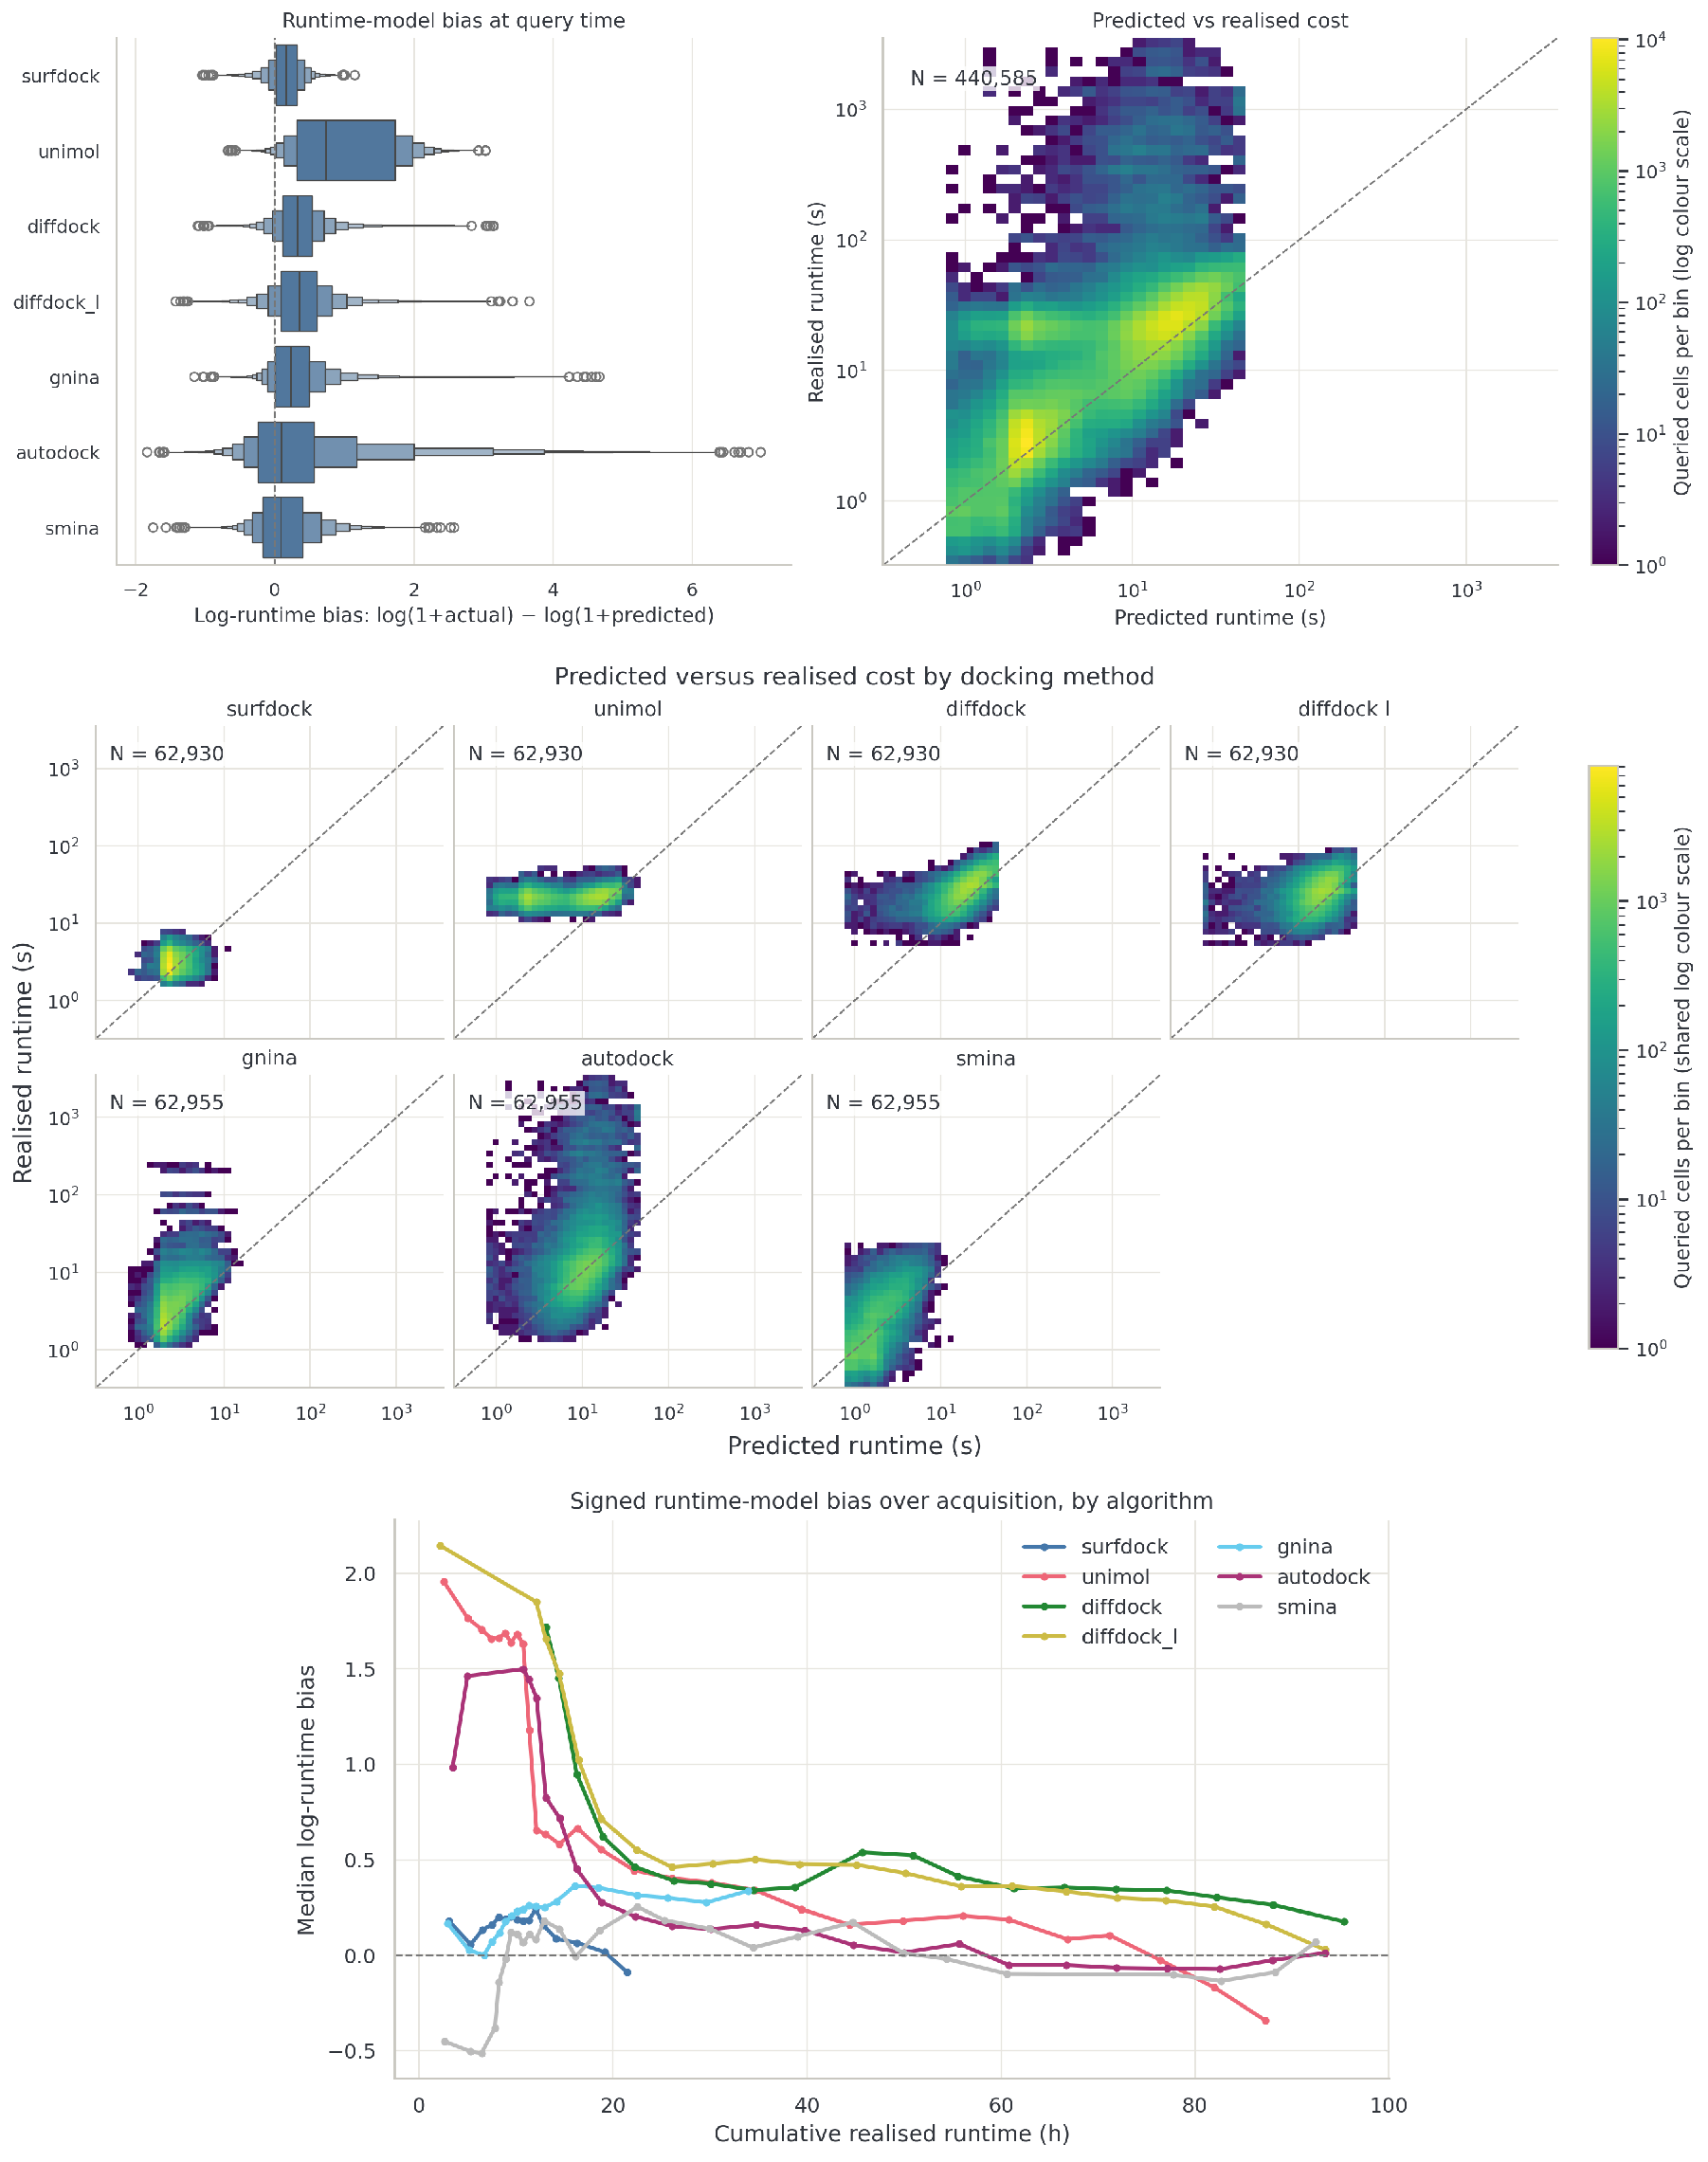
\includegraphics[width=\linewidth]{figures/cost_prediction.pdf}
\caption{Post-warm-start online runtime diagnostics for 440,585 queried-cell records pooled over five cost-aware policies and five folds. Top left: per-algorithm signed log-runtime error; positive values denote underprediction. Top right: pooled density of realized versus predicted runtime. Middle: per-algorithm densities. Bottom: within-bin median signed error over cumulative realized cost. Records can repeat historical cells across policies and overlapping folds.}
\label{fig:cost_prediction}
\end{figure}

For a queried cell, define the signed error $\log(1+C)-\log(1+\widehat C)$, so positive values denote underprediction. In Figure~\ref{fig:cost_prediction}, excluding warm-start observations, the pooled queried-cell distribution is shifted above zero, although errors differ by engine. Uni-Mol and both DiffDock variants are strongly underpredicted initially, whereas Smina is initially overpredicted; several trajectories approach or cross zero later. AutoDock Vina has a less extreme central bias than Uni-Mol but a longer positive tail, corresponding to rare runtimes far beyond its central predictions. The bottom panel pools policies and folds before forming cumulative-cost bins and reports the within-bin median for each engine.

These records describe acquired cells, not calibration over the unqueried pool. The same historical docking outcome can appear in multiple policies and overlapping training folds, so records are not independent docking measurements. The plots document systematic error but neither identify its cause nor evaluate a correction.

\subsection{Effect of cost awareness on acquisition allocation}
\label{app:acquisition-allocation}

\begin{figure}[htbp]
\centering
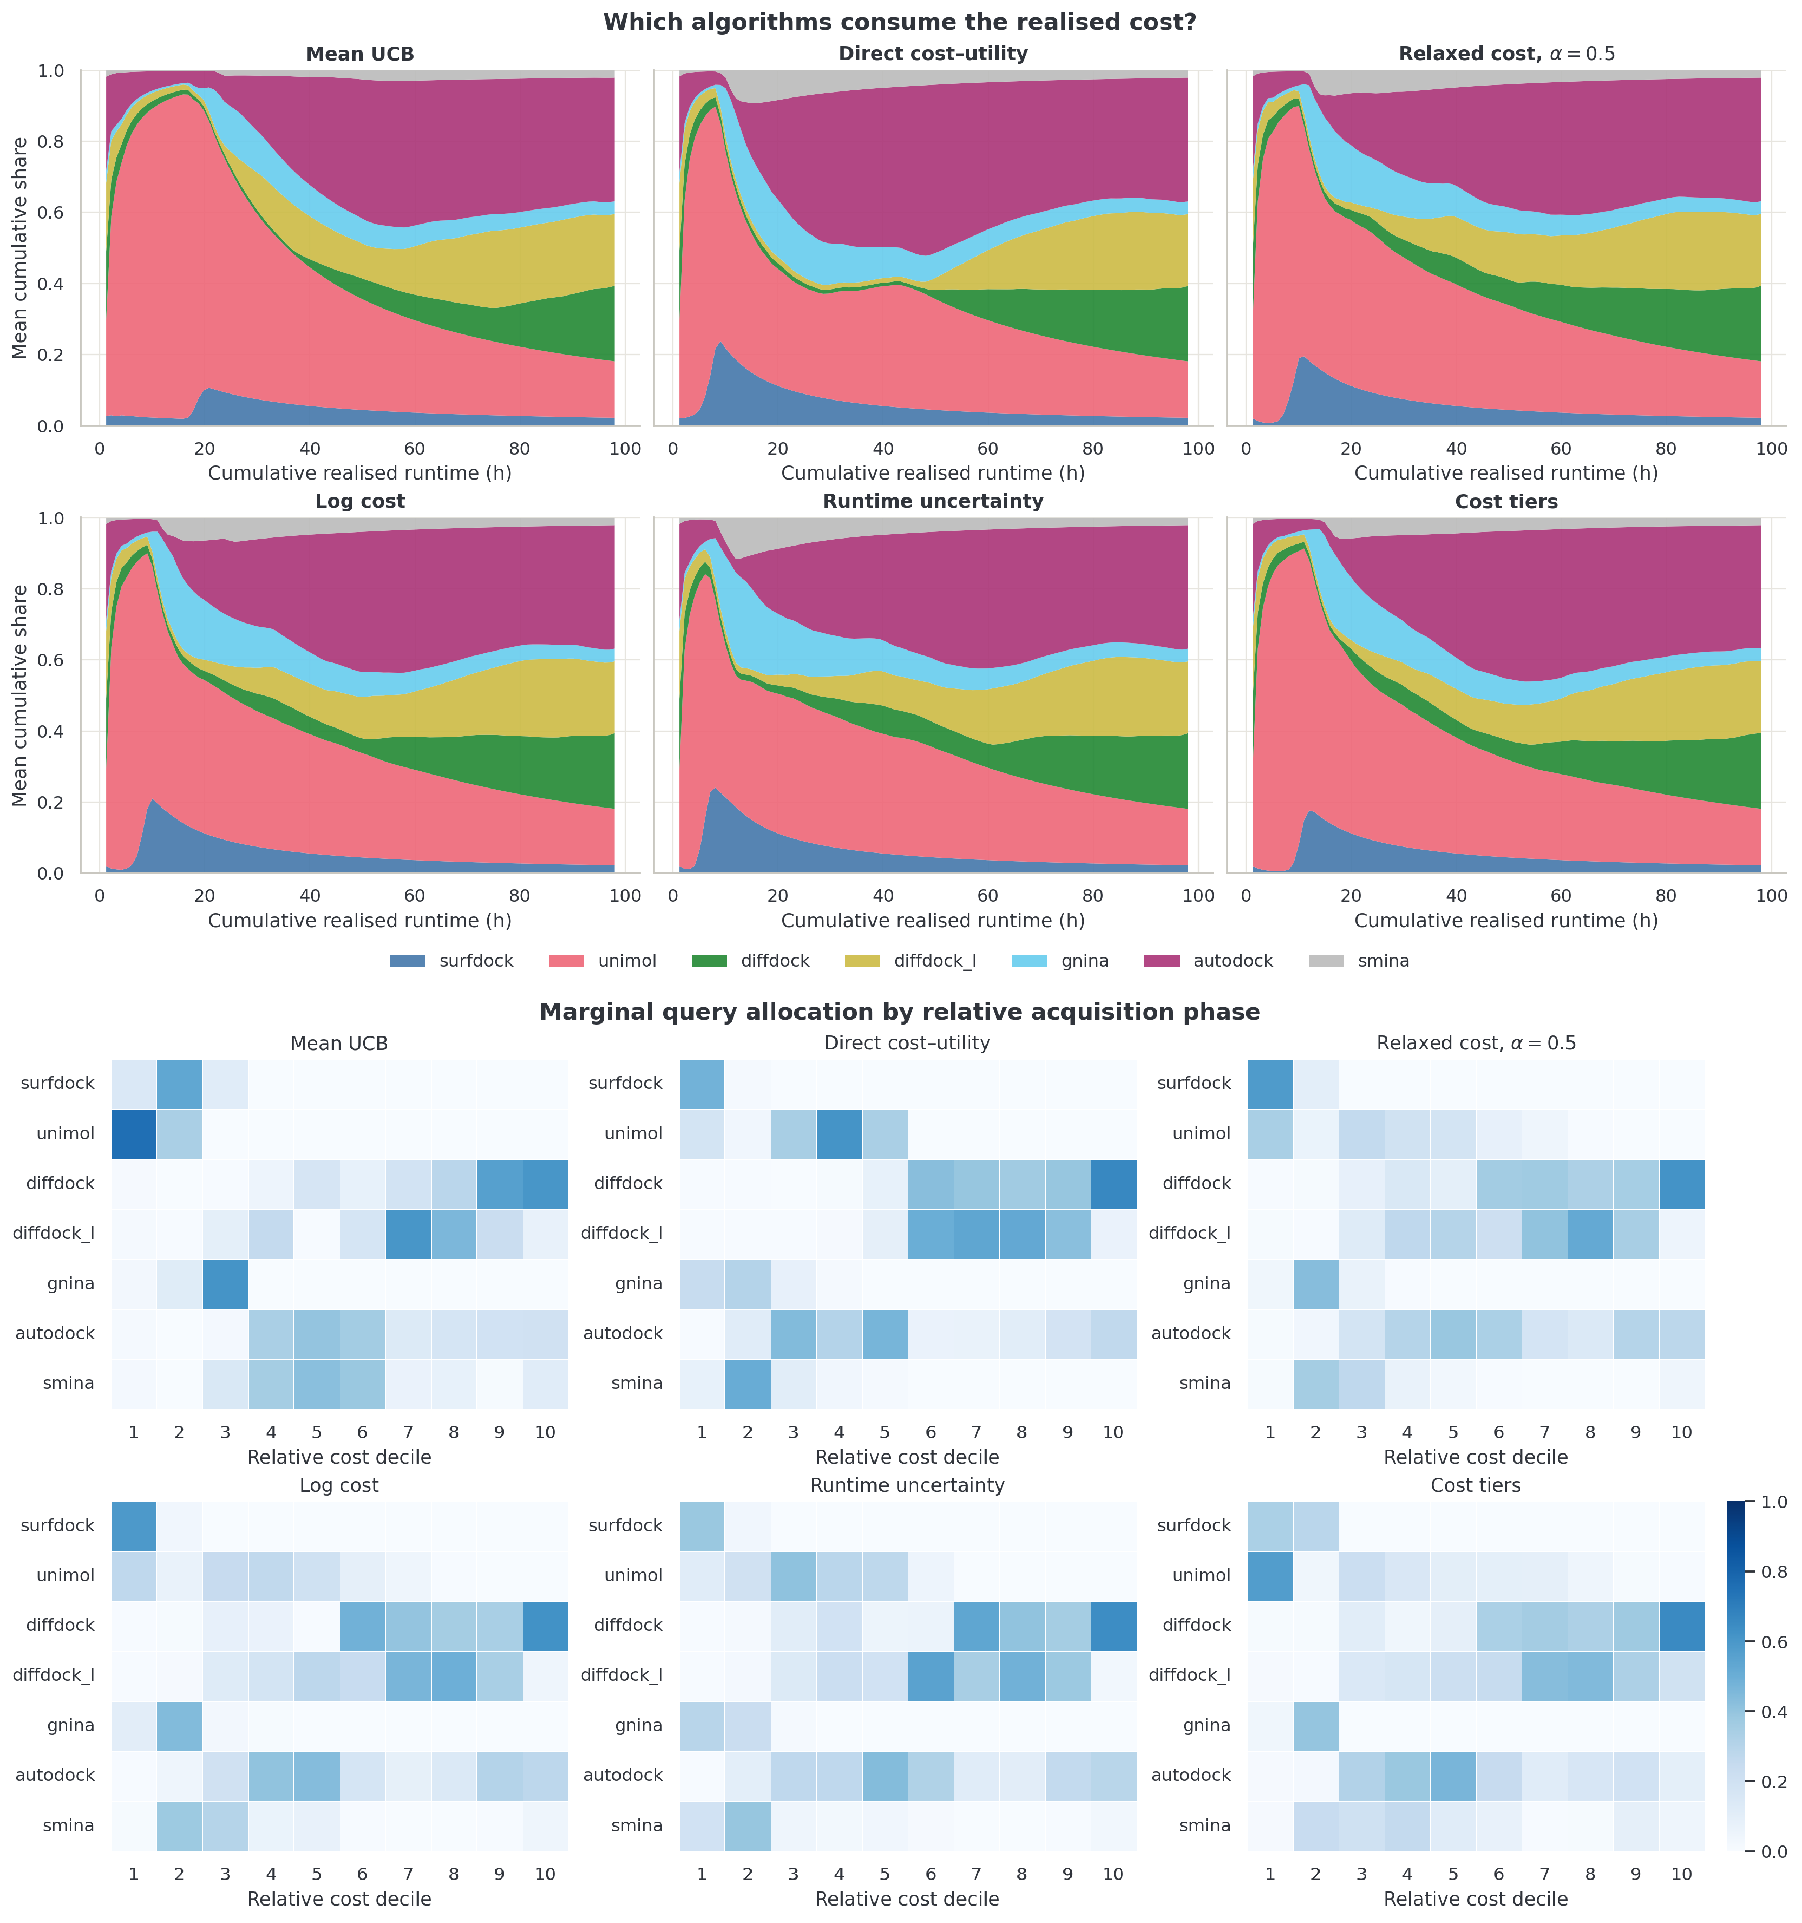
\includegraphics[width=\linewidth]{figures/algorithm_proportion.pdf}
\caption{Top: five-fold mean cumulative realized-cost share by docking engine for each acquisition method. Bottom: fold-mean query share in successive $10\%$ fractions of each fold's full realized training-pool cost.}
\label{fig:algorithm_proportions}
\end{figure}

The common allocation effect is concentrated early (Figure~\ref{fig:algorithm_proportions}). Mean-UCB assigns most first-decile queries to Uni-Mol. The cost-aware variants reduce that concentration to different extents and bring SurfDock, GNINA, and Smina forward. Smina's main query share moves from the middle of the Mean-UCB trajectory to approximately the second or third $10\%$-cost phase. Expensive DiffDock queries are correspondingly deferred. Many cheap Smina queries consume little runtime, while fewer Uni-Mol or extreme AutoDock Vina queries can dominate realized cost. Since every policy eventually observes the same full matrix, these differences describe sequencing.

Signed prediction errors alone do not explain this sequencing. Smina is queried earlier despite early overprediction, whereas Uni-Mol is queried less despite underprediction. This is consistent with coarse between-engine cost separation influencing allocation despite imperfect absolute predictions; it does not show that calibration errors are harmless or establish their causal effect on selector quality.

\begin{figure}[htbp]
\centering
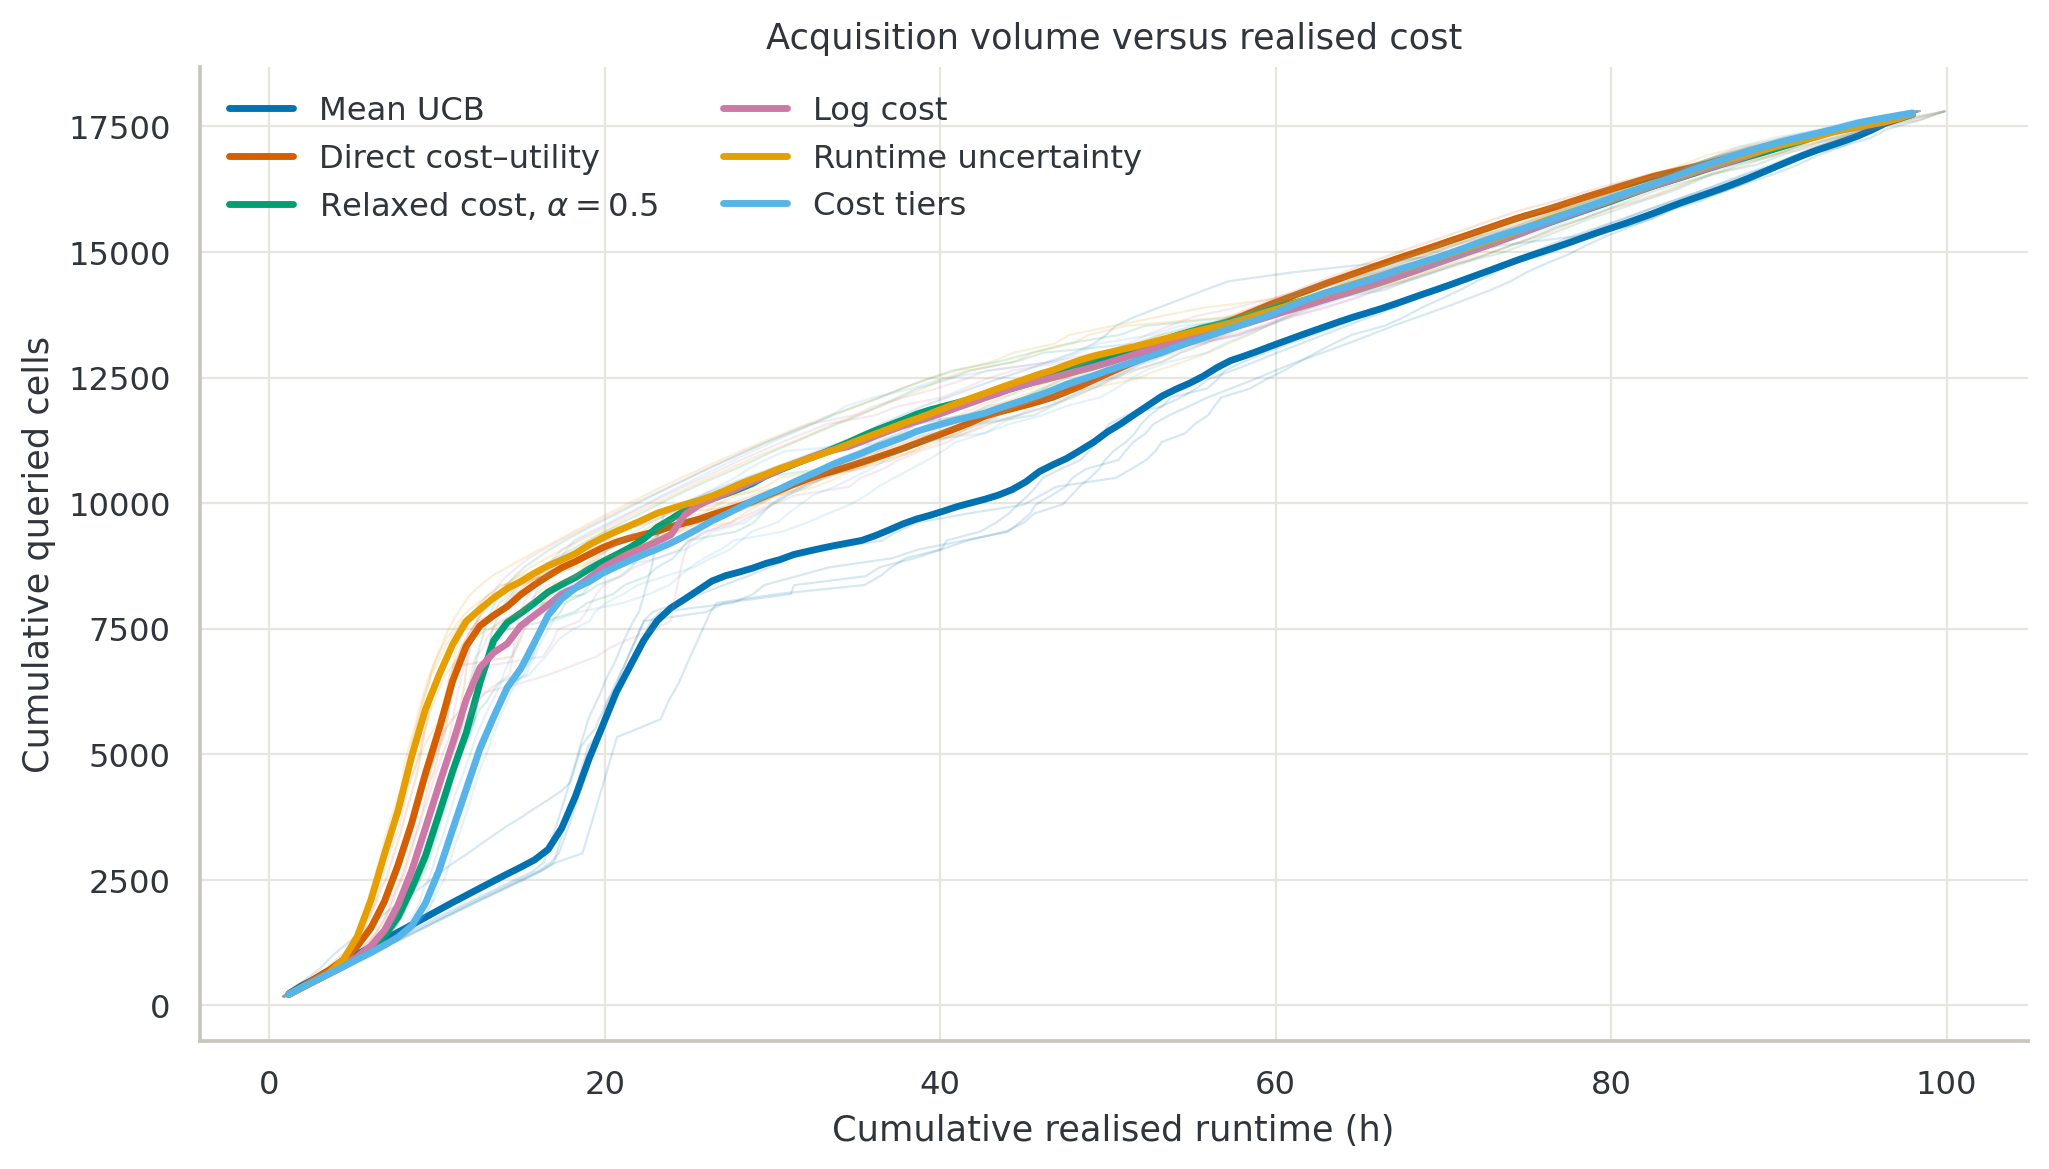
\includegraphics[width=0.75\linewidth]{queried_cells_vs_cost.png}
\caption{Cumulative queried cells versus realized runtime for AL seed~0. Thick curves are five-fold macro means after interpolation over common realized-cost support; faint curves show observed fold trajectories.}
\label{fig:cells2cost}
\end{figure}

Figure~\ref{fig:cells2cost} shows greater acquisition volume for the evaluated cost-aware policies over much of the plotted intermediate-cost range, before convergence when the matrix is exhausted. More acquired cells per realized hour do not by themselves establish greater information value or better downstream decisions.

\begin{figure}[htbp]
\centering
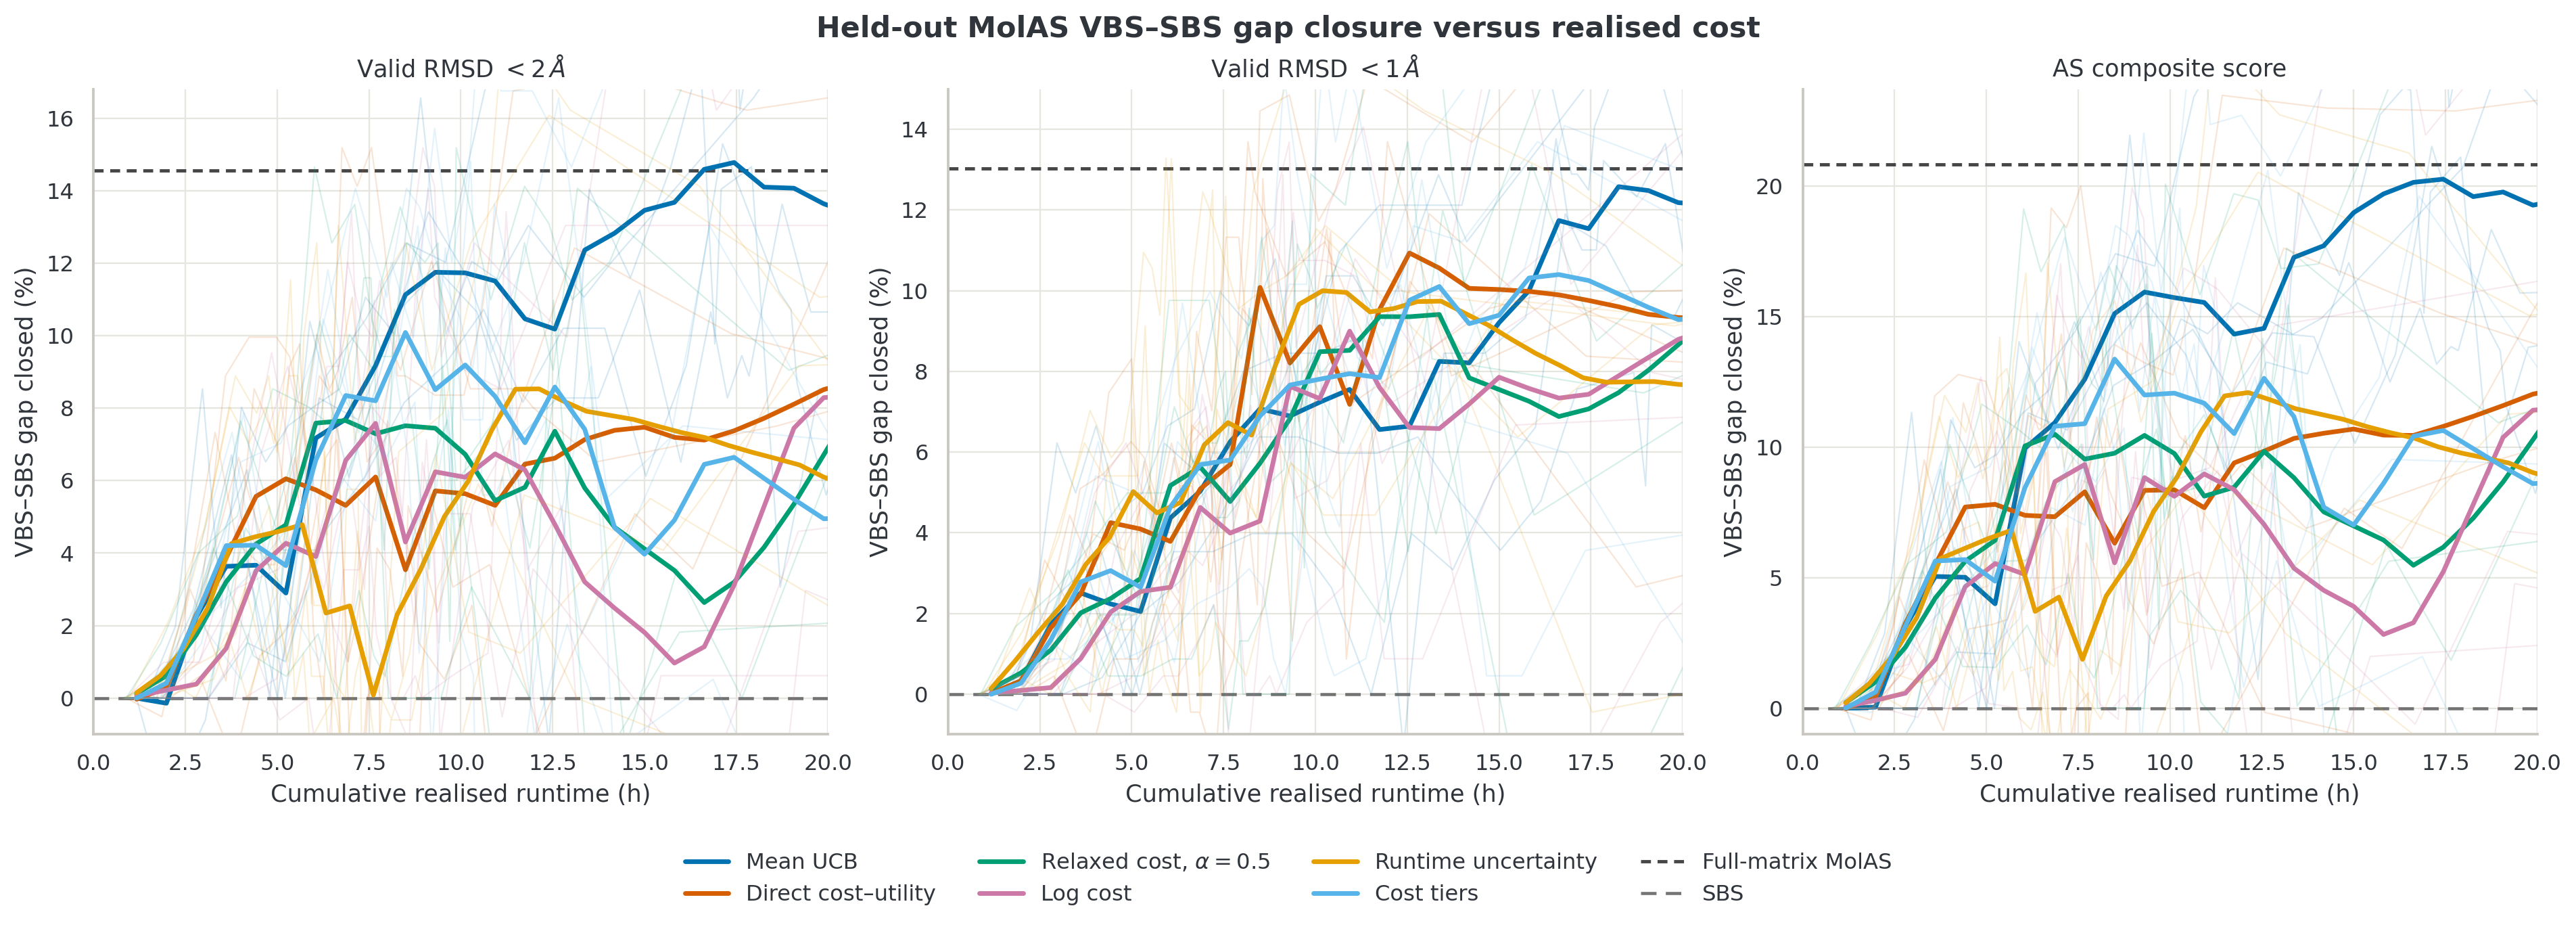
\includegraphics[width=\linewidth]{figures/zoomed_early_downstream_performance_vs_cost.png}
\caption{Held-out SBS--VBS gap closure over the first 20 realized hours. Thick curves are interpolated five-fold macro means; faint curves show fold trajectories. Dashed lines denote SBS ($0\%$ gap closure) and full-matrix MolAS.}
\label{fig:early_downstream}
\end{figure}

Figure~\ref{fig:early_downstream} shows formulation-, endpoint-, and budget-dependent downstream trajectories. Some cost-aware policies exceed the Mean-UCB macro curve over portions of the early-budget range, but these descriptive differences do not establish a statistically significant advantage. Interpolation summarizes evaluated checkpoints; it does not represent a separately trained selector at every plotted runtime. Shared algorithm-level reallocations do not map one-to-one to held-out performance, motivating evaluation of the complete acquisition--completion--selection pipeline.

\subsection{Scope, interpretation, and next steps}
\label{app:next-steps}

Our contribution is an empirical evaluation using established active-learning and matrix-completion methods. The findings concern the evaluated Mean-UCB formulations. Random-cell and pure-uncertainty controls are absent, so improvement over random partial acquisition remains unestablished. Broader comparisons should include joint batch acquisition such as BatchBALD, Pareto-aware policies, and budgeted lookahead. BatchBALD requires joint probabilistic information calculations; SVD disagreement alone is insufficient. The current policies are myopic. These comparisons remain next steps.

MolAS learns from completed targets. An observed-entry-only comparison on identical acquisition histories, using a suitable masked objective, would assess dependence on imputation without treating missing outcomes as failures. Adaptive sampling would still make observed entries selective. Feature-conditioned completion models would test dependence on SVD. Additional acquisition and selector seeds, paired comparisons at prespecified realized-cost checkpoints, and appropriately qualified uncertainty estimates would strengthen statistical characterization. Current fold curves are descriptive, without confidence intervals or formal early-budget significance tests; overlapping training sets and repeated checkpoints are not independent replications. Sensitivity to initialization, $\beta$, SVD ranks, reranking interval, and clipping remains unestablished. These settings define the evaluated configuration rather than validated deployment defaults.

The runtime diagnostics document engine-specific bias on acquired cells, without establishing calibration over the unqueried pool or validating a correction. Calibration using only previously revealed outcomes is a next step, assessed with predictions recorded before each outcome is revealed. Its effects on acquisition and downstream quality require separate evaluation. Guidance on endpoint/budget selection, validation, and monitoring should not be interpreted as an empirically validated stopping or calibration procedure.

Additional datasets, protein--ligand domains, and portfolios would test external validity. Prospective docking is needed to assess hardware transfer, runtime drift, failures, timeouts, retries, and parallel execution. Historical replay does not establish these operational properties, and pose-quality endpoints do not establish experimental hit-discovery benefits. Conclusions remain restricted to the reported retrospective evidence.

\end{document}
